\documentclass[11pt]{article}
\usepackage[margin=2.5cm]{geometry}
\usepackage{graphicx}
\usepackage{booktabs}
\usepackage{amsmath}
\usepackage{caption}
\usepackage[colorlinks=true,linkcolor=blue,citecolor=blue]{hyperref}

\title{Turn-Taking and Leadership Analysis of the Evolved Hebbian Flocking Controller\\
\large Methodology and Simulation Results Summary}
\author{}
\date{\today}

\begin{document}
\maketitle

\noindent This document summarizes the evolutionary training methodology, simulation conditions,
evaluation protocol, and turn-taking/leadership metrics computed for the three
\texttt{hardware\_transfer\_test} conditions (rule-based baseline, pre-safety-layer evolved
controller, safety-layer evolved controller), building on Mahdavi et al.'s ANTS 2026 paper
\emph{``Energy-Efficient Flocking in Self-Organized Robot Swarms''} \cite{mahdavi2026}. It is
written to be dropped into an Overleaf
project as-is (compile with \texttt{pdflatex}) or cannibalized section-by-section into a
Methodology / Simulation Results write-up. All figures referenced below live in
\texttt{figures/} alongside this file, each exported as \texttt{.pdf} (vector, used by
\texttt{\textbackslash includegraphics} below), \texttt{.svg} (for further editing), and
\texttt{.png} (for quick preview outside LaTeX).

\section*{Figure import guide}
\begin{center}
\begin{tabular}{@{}lll@{}}
\toprule
\textbf{File (basename, no extension)} & \textbf{Content} & \textbf{Used in} \\
\midrule
\texttt{paper\_fig5a\_distance\_vs\_battery\_n10} & Fig.~5a analog & \S\ref{sec:paper-figs} \\
\texttt{paper\_fig6\_trajectory\_comparison} & Fig.~6 analog & \S\ref{sec:paper-figs} \\
\texttt{safety\_clamp\_scale\_function} & clamp scale function $C(g)$ & \S\ref{sec:clamp-formula} \\
\texttt{metric3\_front\_occupancy} & front-rank occupancy \& flatness & \S\ref{sec:metric3} \\
\texttt{metric3\_exchange\_rate} & raw exchange rate vs.\ swarm size & \S\ref{sec:metric3} \\
\texttt{metric3\_front\_id\_timeline\_n10} & raw front-identity timeline & \S\ref{sec:metric3} \\
\texttt{metric3\_seed\_sweep\_n10} & occupancy flatness, 30 seeds & \S\ref{sec:metric3} \\
\texttt{metric4\_exchange\_rate\_filtered} & filtered exchange rate vs.\ swarm size & \S\ref{sec:metric4} \\
\texttt{metric4\_handoff\_timeline\_n10} & filtered hand-off timeline & \S\ref{sec:metric4} \\
\texttt{metric4\_switch\_event\_raster\_n10} & hand-off timing, 30 seeds & \S\ref{sec:metric4} \\
\texttt{metric4\_seed\_sweep\_n10} & real hand-off count, 30 seeds & \S\ref{sec:metric4} \\
\bottomrule
\end{tabular}
\end{center}

\section{Methodology}

\subsection{Controller representation and evolutionary training}
\label{sec:evolution}
This subsection documents the design choices behind \emph{how the two evolved genomes
(pre-clamp and safety-clamp) were produced} in the first place -- distinct from
\S\ref{sec:env}--\ref{sec:metrics-def}, which document how they were subsequently
\emph{evaluated}. Both genomes share the same architecture, sensor model, and CMA-ES
configuration; they differ only in the curriculum they were trained under
(\S\ref{sec:curriculum}) and, for safety-clamp, having the hard safety layer of
\S\ref{sec:clamp-formula} active \emph{during} training rather than only at evaluation time.

\paragraph{Controller: a Hebbian-plasticity MLP.} Each agent runs an identical-architecture,
independently-weighted 10-10-10-2 network (10 sensory inputs, two 10-unit ReLU hidden layers,
a 2-unit $\tanh$ output mapped to $(v,\omega)$). Network weights are \emph{not} themselves
evolved; they start uniform-random in $[-1,1]$ at the beginning of every episode and are
updated online, every step, by a per-synapse Hebbian rule with four evolved coefficients
$(A,B,C,D)$ per synapse:
\begin{equation}
\Delta w_{ij} \;=\; \mu \,\big(A_{ij}\, n_i n_j \;+\; B_{ij}\, n_i \;+\; C_{ij}\, n_j \;+\; D_{ij}\big), \qquad \mu = 0.1,
\label{eq:hebbian-update}
\end{equation}
where $n_i, n_j$ are the pre-/post-synaptic activations either side of weight $w_{ij}$, followed
by clipping the whole weight matrix by its own max-abs value whenever that exceeds 1 (preventing
unbounded growth without otherwise touching sub-unity weights). \textbf{It is the $(A,B,C,D)$
coefficients -- not the network weights themselves -- that CMA-ES evolves}: $4 \times (10{\times}10 + 10{\times}10 + 10{\times}2) = 880$ real-valued genes per genome, bounded to $[-5, 5]$.

\paragraph{Sensor model.} Ten inputs per agent, all normalized to roughly $[-1,1]$: the
distance and bearing to the nearest other agent in each of the four body-relative quadrants
(front/back/left/right, split at $\pm45^\circ$ from heading), the agent's own battery level, and
its own compass heading. Neighbors are only sensed within radius $R=2.01$\,m; quadrants with no
neighbor in range report the sensing radius itself as the ``distance'' (a saturated, not
missing, reading).

\paragraph{CMA-ES configuration.} Table~\ref{tab:cmaes} lists the optimizer settings, identical
for every stage and every genome reported in this document.

\begin{table}[h]
\centering
\caption{CMA-ES configuration (\texttt{optimize\_hebbian.py}).}
\label{tab:cmaes}
\begin{tabular}{@{}ll@{}}
\toprule
Setting & Value \\
\midrule
Population size $\lambda$ & 30 \\
Generations per stage & 100 \\
Initial step size $\sigma_0$ & 0.3 \\
Search-space bounds & $[-5, 5]^{880}$ \\
Fitness per candidate & median efficiency over 3 independent-seed repeats \\
Candidate evaluation swarm size & $n_{\text{agents}}=20$ \\
Candidate evaluation wind grid & $50\times50$ (cost-reduced from the default $200\times200$; a full 3-stage run still takes $\mathcal{O}(10\,\text{h})$) \\
\bottomrule
\end{tabular}
\end{table}

Taking the \emph{median} of 3 repeats (rather than, say, the mean or a single evaluation) follows
the paper's own \texttt{evaluateABCD.m} technique, and exists to stop CMA-ES from rewarding
candidates that just got a lucky spawn configuration once.

\subsubsection{Three-stage curriculum}
\label{sec:curriculum}
Both genomes were trained with the same three sequential stages, each stage's population
seeded from the \emph{previous} stage's single best genome (stage 1 alone starts from a fresh
genome sampled uniformly from $[-5,5]^{880}$) -- a curriculum, not three independent runs:

\begin{enumerate}
\item \textbf{\texttt{walk\_left}} -- wind disabled; fitness is distance travelled only. Teaches
  basic forward locomotion before anything else is asked of the controller.
\item \textbf{\texttt{save\_battery\_avoid\_wall}} -- wind enabled; adds a battery-preservation
  term and a wall-collision penalty (inter-robot collisions not yet penalized).
\item \textbf{\texttt{save\_battery\_avoid\_all}} -- as above, plus an inter-robot collision
  penalty. This is the stage whose output is the genome actually evaluated throughout this
  document.
\end{enumerate}

\noindent Each stage's fitness is
\begin{equation}
\text{eff} = w_d \cdot \text{dist} \;+\; \frac{\overline{\text{batt}}}{w_b} \;-\; \frac{\text{coll} + m_w \cdot \text{wall\_coll}}{w_c},
\label{eq:stage-fitness}
\end{equation}
with the per-stage weights in Table~\ref{tab:stage-weights} (a blank entry means that term is
absent for that stage, matching the paper's Table 2 having no battery/collision terms for stage
1, etc.) and $w_d=16.0$ applied uniformly across all three stages.

\begin{table}[h]
\centering
\caption{Per-stage fitness weights in Eq.~\ref{eq:stage-fitness} ($w_c$'s wall multiplier $m_w=3.0$ throughout).}
\label{tab:stage-weights}
\begin{tabular}{@{}lccc@{}}
\toprule
Stage & $w_b$ (battery) & $w_c$ (collision) & incl.\ inter-robot term? \\
\midrule
\texttt{walk\_left} & -- & -- & -- \\
\texttt{save\_battery\_avoid\_wall} & 5.0 & 500.0 & no (wall only) \\
\texttt{save\_battery\_avoid\_all} & 5.0 & 250.0 & yes \\
\bottomrule
\end{tabular}
\end{table}

\paragraph{A disclosed deviation: the distance weight $w_d$.} The paper's Table 2 formula has
no explicit distance weight (implicitly $w_d=1$). Early training runs under that literal
formula let CMA-ES discover a degenerate optimum: distance travelled collapsed from
$\approx$84\,m (stage 1, no battery term to compete with) to $\approx$1.5--1.6\,m once the
battery term was introduced, because barely moving is a cheap way to preserve battery once
distance stops dominating the score. $w_d=16.0$ was reached empirically, mirroring the
LJ-baseline model's own identical fix for the identical failure mode: starting from the LJ
model's calibrated value of 8.0 as a reasoned prior, then sweeping $w_d \in \{4, 8, 16, 32\}$
(3 seeds each, $n=10$) and selecting 16.0 as the clear winner on both collision time and
battery, with 32.0 regressing part of the way back toward 8.0's behavior. This is a deliberate,
disclosed deviation from Table 2's literal formula, not a claim of exact replication.

\subsubsection{Why two separately-trained genomes: the safety-layer investigation}
\label{sec:why-two-genomes}
The pre-clamp genome (trained under the curriculum above with none of \S\ref{sec:clamp-formula}'s
mechanisms active) was observed to spend a large fraction of its episode in chronic inter-agent
collision, burning battery with no offsetting benefit, despite covering statistically the same
distance as the rule-based baseline. Several fixes were tried \emph{before} arriving at the
safety-clamp design reported in this document, each evaluated across multiple seeds where noted:
tightening the collision-penalty weight alone (fixed collisions but made battery worse -- the
tight, colliding formation was apparently providing an incidental wind-shielding benefit that
disappeared with nothing to replace it); adding a small cohesion reward on top of the collision
fix (worked on one seed, failed or reversed on two others); and physically preventing overlap at
full strength (battery cratered further, and the controller commanded \emph{more} collision-course
moves than any other variant tried -- removing the physical consequence of crowding entirely
seems to remove the only signal teaching the controller to avoid it). \textbf{A hard, non-learned
forward-speed clamp} (\S\ref{sec:clamp-formula}) combined with a training-time sim-to-real
minimum-distance margin and a \emph{soft} (partial, not full) collision-resolution push was the
combination that finally produced genuinely low inter-robot collision without the battery or
gridlock regressions the other attempts showed.

Critically, this combination was \textbf{retrained from scratch through the full curriculum}
rather than bolted onto the existing pre-clamp genome: a pilot test applying the clamp to an
already-trained genome that had never experienced it caused distance to collapse to
$\sim$0--1.5\,m and collision time to explode, as the controller kept commanding full-speed
moves into neighbors, got braked, and gridlocked in a standoff for the rest of the episode.
CMA-ES needs to experience the clamp's consequences \emph{during} evolution to learn to route
around it, rather than have it imposed after the fact.

\subsection{Simulation environment}
\label{sec:env}
All three conditions share the same underlying kinematic/wind/battery physics (a Python port
of the paper's MATLAB reference model). Table~\ref{tab:env} lists the constants common to
every run reported here.

\begin{table}[h]
\centering
\caption{Shared simulation parameters (\texttt{ants26\_replication/experiment/config.py}).}
\label{tab:env}
\begin{tabular}{@{}llp{7cm}@{}}
\toprule
Parameter & Value & Notes \\
\midrule
Time step $\Delta t$ & 0.5\,s & \\
Robot radius & 0.055\,m & \\
Wind-occlusion radius & 0.15\,m & radius used by the wake ray-tracer \\
Arena $Y$ bounds & $[-5, 5]$\,m & hard walls \\
Arena $X$ behavior & shifting 10\,m tracking window & agents fly indefinitely in $-x$; window follows the swarm's leading edge (max span 9.8\,m) \\
Freestream wind speed $v_{\text{wind}}$ & 10.0 & \\
Freestream power $U_\infty$ & 100.0 & wake ray-tracing input \\
Drag scale $\kappa$ & 10.0 & \\
Wind grid resolution ($N_x{\times}N_y$) & \textbf{50$\times$50} & see \S\ref{sec:protocol} -- NOT config.py's default of 200 \\
Spawn region & 3\,m square about $(0,0)$ & min.\ pairwise spawn gap 0.1\,m + $2r$ \\
Collision threshold (min.\ pairwise dist.) & $0.01 + 2r = 0.12$\,m & before any per-condition inflation (\S\ref{sec:conditions}) \\
Linear speed limit & 0.20\,m/s & \\
Angular speed limit & $\pi/5$\,rad/s & \\
\bottomrule
\end{tabular}
\end{table}

\subsection{Compared conditions}
\label{sec:conditions}

\paragraph{LJ baseline (Table 3, rule-based).} The paper's ``standard collective motion''
comparison point: a fixed Lennard-Jones spacing force + heading-alignment force + goal-pull
force, mapped to a (linear, angular) velocity command -- no learning, no battery awareness.
Table~\ref{tab:lj} gives the exact gains (from
\texttt{hardware\_transfer\_test/lj\_baseline/paper\_baseline\_rules.json}, identical to
\texttt{config.PAPER\_BASELINE\_RULES}). Battery is on this model's own native 0--150 scale
(every trained-genome condition below uses 0--100); all battery percentages reported in this
document are normalized to \% of full charge so the three conditions are directly comparable.

\begin{table}[h]
\centering
\caption{LJ baseline control-law parameters.}
\label{tab:lj}
\begin{tabular}{@{}lll@{}}
\toprule
Parameter & Value & Parameter \quad Value \\
\midrule
$r_0$ (LJ equilibrium spacing) & 0.7\,m & $K_1$ (linear-vel.\ gain) \quad 0.05 \\
$\epsilon$ (LJ well depth) & 1.0 & $K_2$ (angular-vel.\ gain) \quad 0.5 \\
$k_{\text{align}}$ (heading-alignment gain) & 0.0 & $U$ (forward-speed bias) \quad 0.0 \\
$k_{\text{goal}}$ (goal-pull gain) & 3.0 & \\
\midrule
$r_{\text{cut}}$ (LJ interaction cutoff) & 3.0\,m & $r_{\text{min}}$ (singularity guard) \quad 0.0\,m \\
$R_{\text{align}}$ (alignment neighbor radius) & 1.5\,m & Battery scale \quad 0--150 \\
\bottomrule
\end{tabular}
\end{table}

\paragraph{Pre-clamp (evolved, no safety layer).} A Hebbian ABCD controller: a 10-input,
two-hidden-layer (10 units each), 2-output ($v,\omega$) network whose weights are updated
online by a per-synapse Hebbian rule with 4 coefficients per synapse ($A,B,C,D$), themselves
evolved by CMA-ES -- 880 evolved parameters total. Trained via the paper's 3-stage curriculum
(\texttt{walk\_left} $\to$ \texttt{save\_battery\_avoid\_wall} $\to$
\texttt{save\_battery\_avoid\_all}), $n_{\text{agents}}=20$, seed 42, wind grid $50{\times}50$,
battery sensor enabled, \emph{before} any of the safety mechanisms below existed
(training run \texttt{n20\_3stage}, best in-training efficiency score 201.9). Genome file:
\texttt{hardware\_transfer\_test/pre\_clamp\_best/genome\_trained\_n20.npy}.

\paragraph{Safety-clamp (evolved + hard reflex).} The same architecture and curriculum,
\emph{re-trained from scratch with three additional non-learned safety mechanisms active
during training itself} (training run \texttt{n20\_safety\_full3stage2}, same seed/n\_agents/wind
grid, best in-training efficiency score 434.6 -- more than double the pre-clamp genome's, on
the in-training fitness scale, though the two are not runs of the identical fitness formula
version and so are not directly comparable as a single number). Genome file:
\texttt{hardware\_transfer\_test/safety\_clamp\_best/genome\_trained\_n20.npy}. The three
mechanisms (Table~\ref{tab:clamp}):

\begin{table}[h]
\centering
\caption{Safety-clamp condition's additional non-learned mechanisms.}
\label{tab:clamp}
\begin{tabular}{@{}lp{10cm}@{}}
\toprule
Mechanism & Parameters \\
\midrule
Hard forward-speed clamp (agent-agent) & Full speed above 0.30\,m gap; linearly brakes to zero forward speed at 0.05\,m gap. Uses the true robot radius (not inflated). Turning is left unaffected. \\
Hard forward-speed clamp (agent-wall) & Full speed above 0.15\,m gap to a wall; zero at 0.02\,m gap. \\
Sim-to-real min.\ distance inflation & Collision counting / instant-death / proximity-penalty bookkeeping (training-time only) treats agents as $1.3\times$ their true size, so CMA-ES leaves a physical safety margin once evaluated at true size. \\
Soft collision resolution & When agents nonetheless end a step overlapping, they are pushed apart by 50\% of the remaining gap-to-\texttt{min\_dist}, for up to 2 passes per step (a partial, not full, physical de-overlap). \\
\bottomrule
\end{tabular}
\end{table}

\subsubsection{How the forward-speed clamp works}
\label{sec:clamp-formula}
The clamp (\texttt{\_apply\_safety\_clamp()} in \texttt{simulation\_hebbian.py}) is applied to
every agent at every simulation step, \emph{before} kinematic integration, using that step's
pre-integration positions. It rescales only the commanded \emph{forward} speed $v_i$ output by
the network -- the angular command $\omega_i$ passes through unchanged, so a braked agent can
still turn away. Define the piecewise-linear scale function, for a surface gap $g \geq 0$ and
thresholds $g_{\text{in}} < g_{\text{out}}$:
\begin{equation}
C(g;\, g_{\text{in}}, g_{\text{out}}) \;=\; \operatorname{clip}\!\left(\frac{g - g_{\text{in}}}{g_{\text{out}} - g_{\text{in}}},\; 0,\; 1\right)
\;=\;
\begin{cases}
0 & g \leq g_{\text{in}} \\[2pt]
\dfrac{g - g_{\text{in}}}{g_{\text{out}} - g_{\text{in}}} & g_{\text{in}} < g < g_{\text{out}} \\[6pt]
1 & g \geq g_{\text{out}}
\end{cases}
\label{eq:clamp-scale}
\end{equation}
i.e.\ full speed above $g_{\text{out}}$, a linear ramp down to zero at $g_{\text{in}}$, and zero
(full stop) at or below $g_{\text{in}}$ (Fig.~\ref{fig:clamp-formula}). Two instances of
Eq.~\ref{eq:clamp-scale} are evaluated per agent per step, using the \emph{true},
uninflated robot radius $r=0.055$\,m in both:
\begin{align}
g_i^{\text{agent}} &= \min_{j \neq i} \big(\lVert p_i - p_j \rVert - 2r\big)
&&\text{(gap to the nearest other agent's surface)} \\
g_i^{\text{wall}} &= \min\big(y_{\text{top}} - y_i,\; y_i - y_{\text{bottom}}\big)
&&\text{(gap to the nearer of the two $Y$ walls)}
\end{align}
and the more restrictive of the two scales the commanded forward speed:
\begin{equation}
v_i^{\text{clamped}} \;=\; v_i^{\text{cmd}} \cdot \min\Big(
C\big(g_i^{\text{agent}};\, 0.05,\, 0.30\big),\;
C\big(g_i^{\text{wall}};\, 0.02,\, 0.15\big)
\Big)
\label{eq:clamp-combined}
\end{equation}
with the numeric thresholds from Table~\ref{tab:clamp}. The wall thresholds are narrower than
the agent-agent ones because a wall is stationary, so the worst-case single-step closing
distance toward it ($v_{\max}\Delta t = 0.20 \times 0.5 = 0.10$\,m) is half that of two agents
closing head-on ($2 v_{\max}\Delta t = 0.20$\,m).

\begin{figure}[h]
\centering
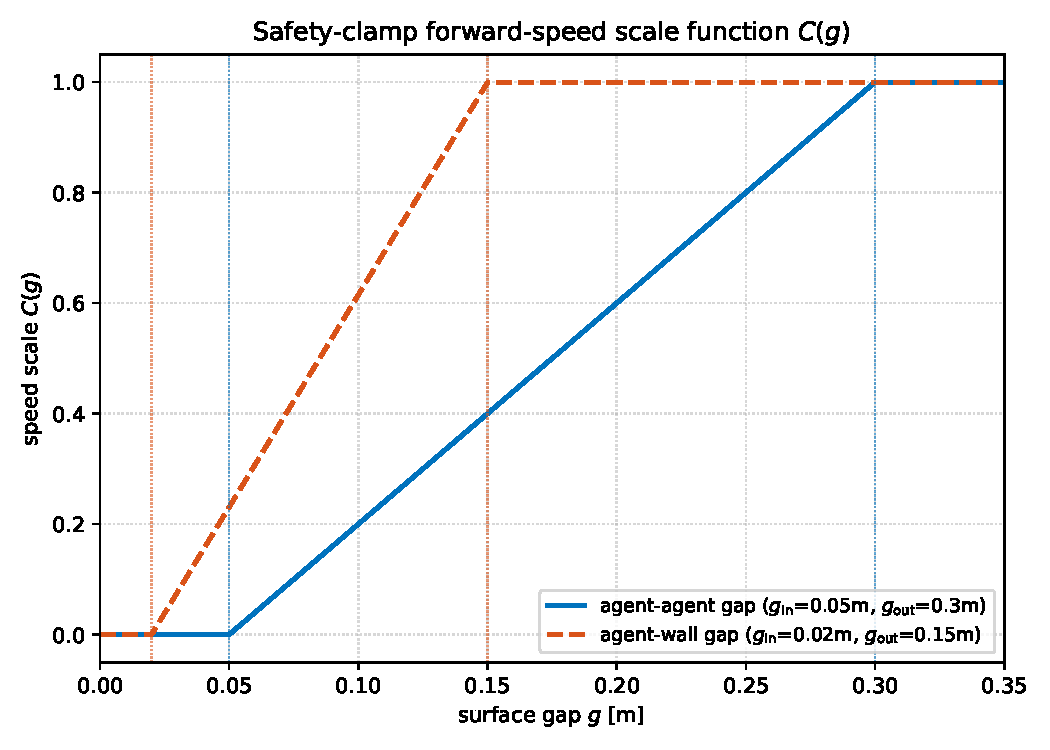
\includegraphics[width=0.7\textwidth]{figures/safety_clamp_scale_function}
\caption{The scale function $C(g)$ (Eq.~\ref{eq:clamp-scale}) for both gap types, with their
respective $g_{\text{in}}$/$g_{\text{out}}$ thresholds marked.}
\label{fig:clamp-formula}
\end{figure}

\subsubsection{The other two mechanisms, briefly}
The sim-to-real minimum-distance inflation simply scales the collision threshold used for
bookkeeping (not for the clamp above, which always uses the true radius):
\begin{equation}
d_{\min} = \big(s + 2r\big) \cdot \kappa, \qquad s = 0.01\,\text{m (slack)},\ \ \kappa = 1.3\ \text{(safety-clamp)}\ \text{or}\ 1.0\ \text{(pre-clamp)}.
\end{equation}
The soft collision-resolution pass, run \emph{after} kinematic integration when a pair still
ends a step with $d_{ij} = \lVert p_i - p_j\rVert < d_{\min}$, moves the lower-priority agent
$j$ of the pair toward (not fully to) $d_{\min}$ along their connecting bearing $\theta = \operatorname{atan2}(\Delta y, \Delta x)$, leaving the higher-priority agent $i$ fixed:
\begin{equation}
p_j \;\leftarrow\; p_i + \big[d_{ij} + \lambda\,(d_{\min} - d_{ij})\big]\,(\cos\theta,\, \sin\theta), \qquad \lambda = 0.5\ \text{(strength)},
\end{equation}
repeated for up to 2 passes per step (safety-clamp condition only; disabled entirely for
pre-clamp, where $d_{\min}=0.12$\,m at $\kappa=1$ is used only for bookkeeping, never enforced
physically). With $\kappa=1.3$ the safety-clamp condition's enforced floor is
$d_{\min}=0.156$\,m; because $\lambda<1$ and only 2 passes are run, this deliberately leaves
some \emph{residual} crowding below that floor after a hard pileup, rather than fully
de-overlapping the pair in one step (per \texttt{config.py}'s own calibration note, an
uninflated $\kappa=1$, $d_{\min}=0.12$\,m test of this same $\lambda$/pass-count combination
converged to $\approx$0.095\,m -- short of, but close to, its floor).

\subsection{Evaluation protocol}
\label{sec:protocol}
\texttt{hardware\_transfer\_test/*/n*/metrics.json} only records scalar episode summaries
(distance, battery, collision counts) -- no per-step trajectory -- so the turn-taking metrics
below required re-simulating each condition from its saved genome/rule file rather than reading
the archive directly. The exact re-simulation settings were reverse-engineered by bisecting
config flags until the regenerated episodes reproduced every field of the archived
\texttt{metrics.json} \emph{bit-for-bit} (confirmed for multiple $n_{\text{agents}}$ values); the
single consequential miss was wind-grid resolution -- both genomes' sibling \texttt{\_history.json}
files record they were trained and archived at $50{\times}50$, not \texttt{config.py}'s present-day
default of $200{\times}200$.

\begin{itemize}
\item \textbf{Headline single-run figures} (Fig.~5a/6 analogs, Metric~3/4 vs.\ swarm size,
  timeline plots): seed 42 (\texttt{config.HEBBIAN\_DEFAULT\_SEED}), $n_{\text{agents}} \in
  \{2,3,4,5,10,20\}$, matching \texttt{hardware\_transfer\_test}'s own sweep exactly.
\item \textbf{Statistical / robustness figures} (seed-sweep panels): 30 additional seeds
  (1000--1029, chosen to not overlap the archived seed 42), $n_{\text{agents}}=10$ held fixed,
  same per-condition config overrides as above.
\end{itemize}

\subsection{Turn-taking metrics}
\label{sec:metrics-def}
Both metrics below are derived from the same underlying signal: at every simulation step, agents
are ranked by their position projected onto the flock's instantaneous heading (the circular mean
of each agent's own movement-direction bearing, itself computed from consecutive position
fixes -- not the simulator's internal body-orientation state). Rank~0 is the front-most
(``leading'', aerodynamically disadvantageous) agent; rank~$N{-}1$ is the rearmost (``trailing'',
drafting-advantaged) agent. \textbf{Metric 3 and Metric 4 are deliberately reported as separate
figures, never overlaid on the same axes}, since they are distinct statistics of that signal with
distinct citations.

\paragraph{Metric 3 -- front-rank occupancy \& raw exchange rate.} For each agent, the fraction
of the episode spent at rank~0 (occupancy fraction); flatness of that distribution across agents
is reported as normalized Shannon entropy ($H/\log N$; 1 = every agent leads an equal share of
the time). The raw exchange rate counts every rank-0 identity change, per second and per metre
travelled -- including single-step flips that may just be positional jitter. This is the same
quantity underlying Mirzaeinia et al.\ (2019)'s greedy leader-replacement heuristic and the
``time-in-front'' leadership tracking used in the stork/pigeon literature \cite{mirzaeinia2019}.

\paragraph{Metric 4 -- persistence-filtered hand-off rate.} The same rank-0 identity series,
run-length-encoded, with any run shorter than 3 steps (1.5\,s) merged into its neighbor before
counting transitions -- i.e.\ a hand-off only counts if the new leader holds the position for at
least 1.5\,s. This is presented explicitly as a \emph{simplified, fixed-threshold proxy} for
Butail \& Porfiri (2019)'s transfer-entropy-based switch detector \cite{butail2019}, \textbf{not}
a re-implementation of their method: their approach fits an optimal change-point partition via
transfer entropy, whereas this is a hand-picked dwell-time threshold. Use Metric 4 as a
noise sanity-check on Metric 3's raw count, not as a rigorous statistical switch-detection claim;
implementing the actual transfer-entropy method is the natural next step if reviewers press on
this point.

\emph{(Two further metrics -- Voelkl et al.\ (2015)'s leading/following reciprocity index and
Nagy et al.\ (2010)'s directional-correlation-delay hierarchy network -- are also implemented in
the same codebase but omitted from this summary at the user's request; see
\texttt{hardware\_transfer\_test/leadership\_metrics.py} for the full set.)}

\section{Simulation Results}

\subsection{Paper-replication figures}
\label{sec:paper-figs}

\begin{figure}[h]
\centering
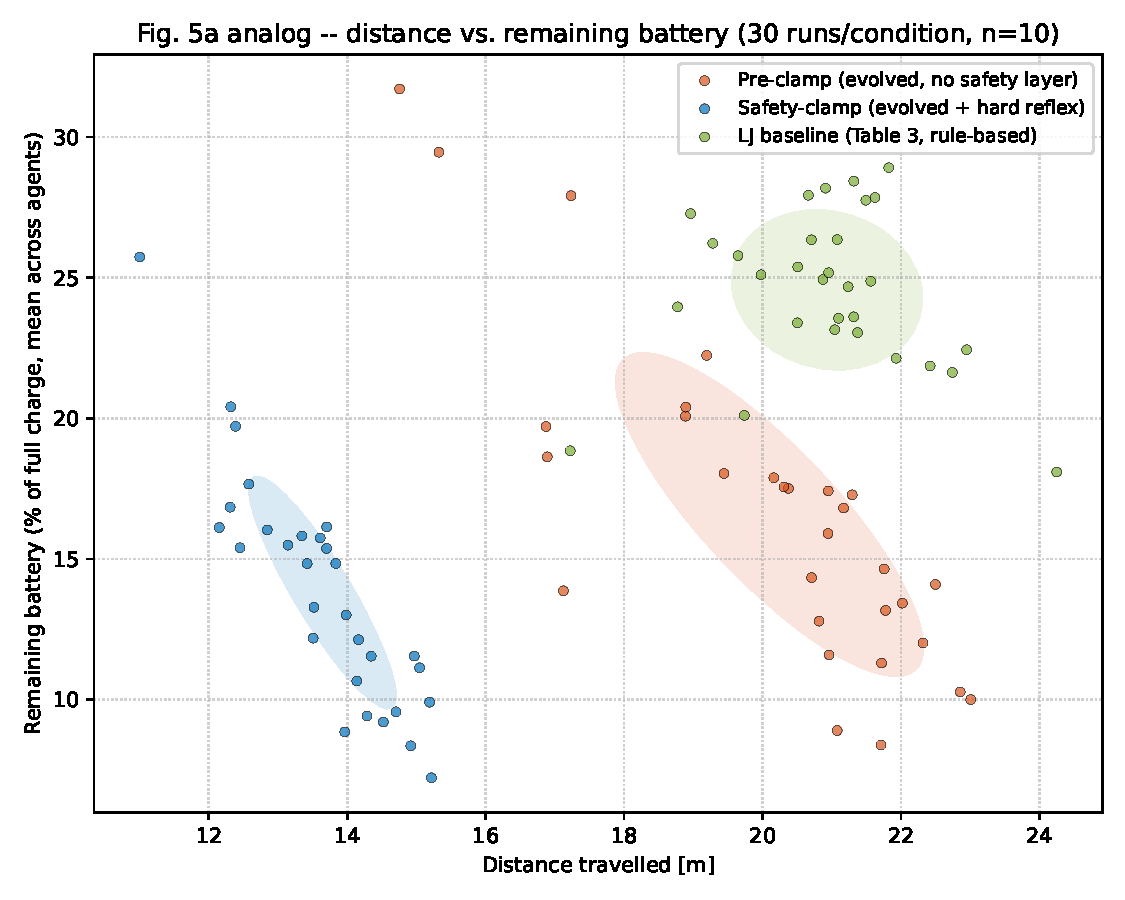
\includegraphics[width=0.85\textwidth]{figures/paper_fig5a_distance_vs_battery_n10}
\caption{\textbf{Fig.~5a analog.} Distance travelled vs.\ remaining battery (\% of full
charge), 30 seeded runs per condition at $n_{\text{agents}}=10$, with 1-std confidence
ellipses (same construction as the paper's original Fig.~5a). The paper's original used 100
runs at its default swarm size; this uses 30 runs (seeds 1000--1029) at $n=10$ for
consistency with the Metric~3/4 seed-sweep figures below, which use the identical 30 runs.}
\label{fig:fig5a}
\end{figure}

\begin{figure}[h]
\centering
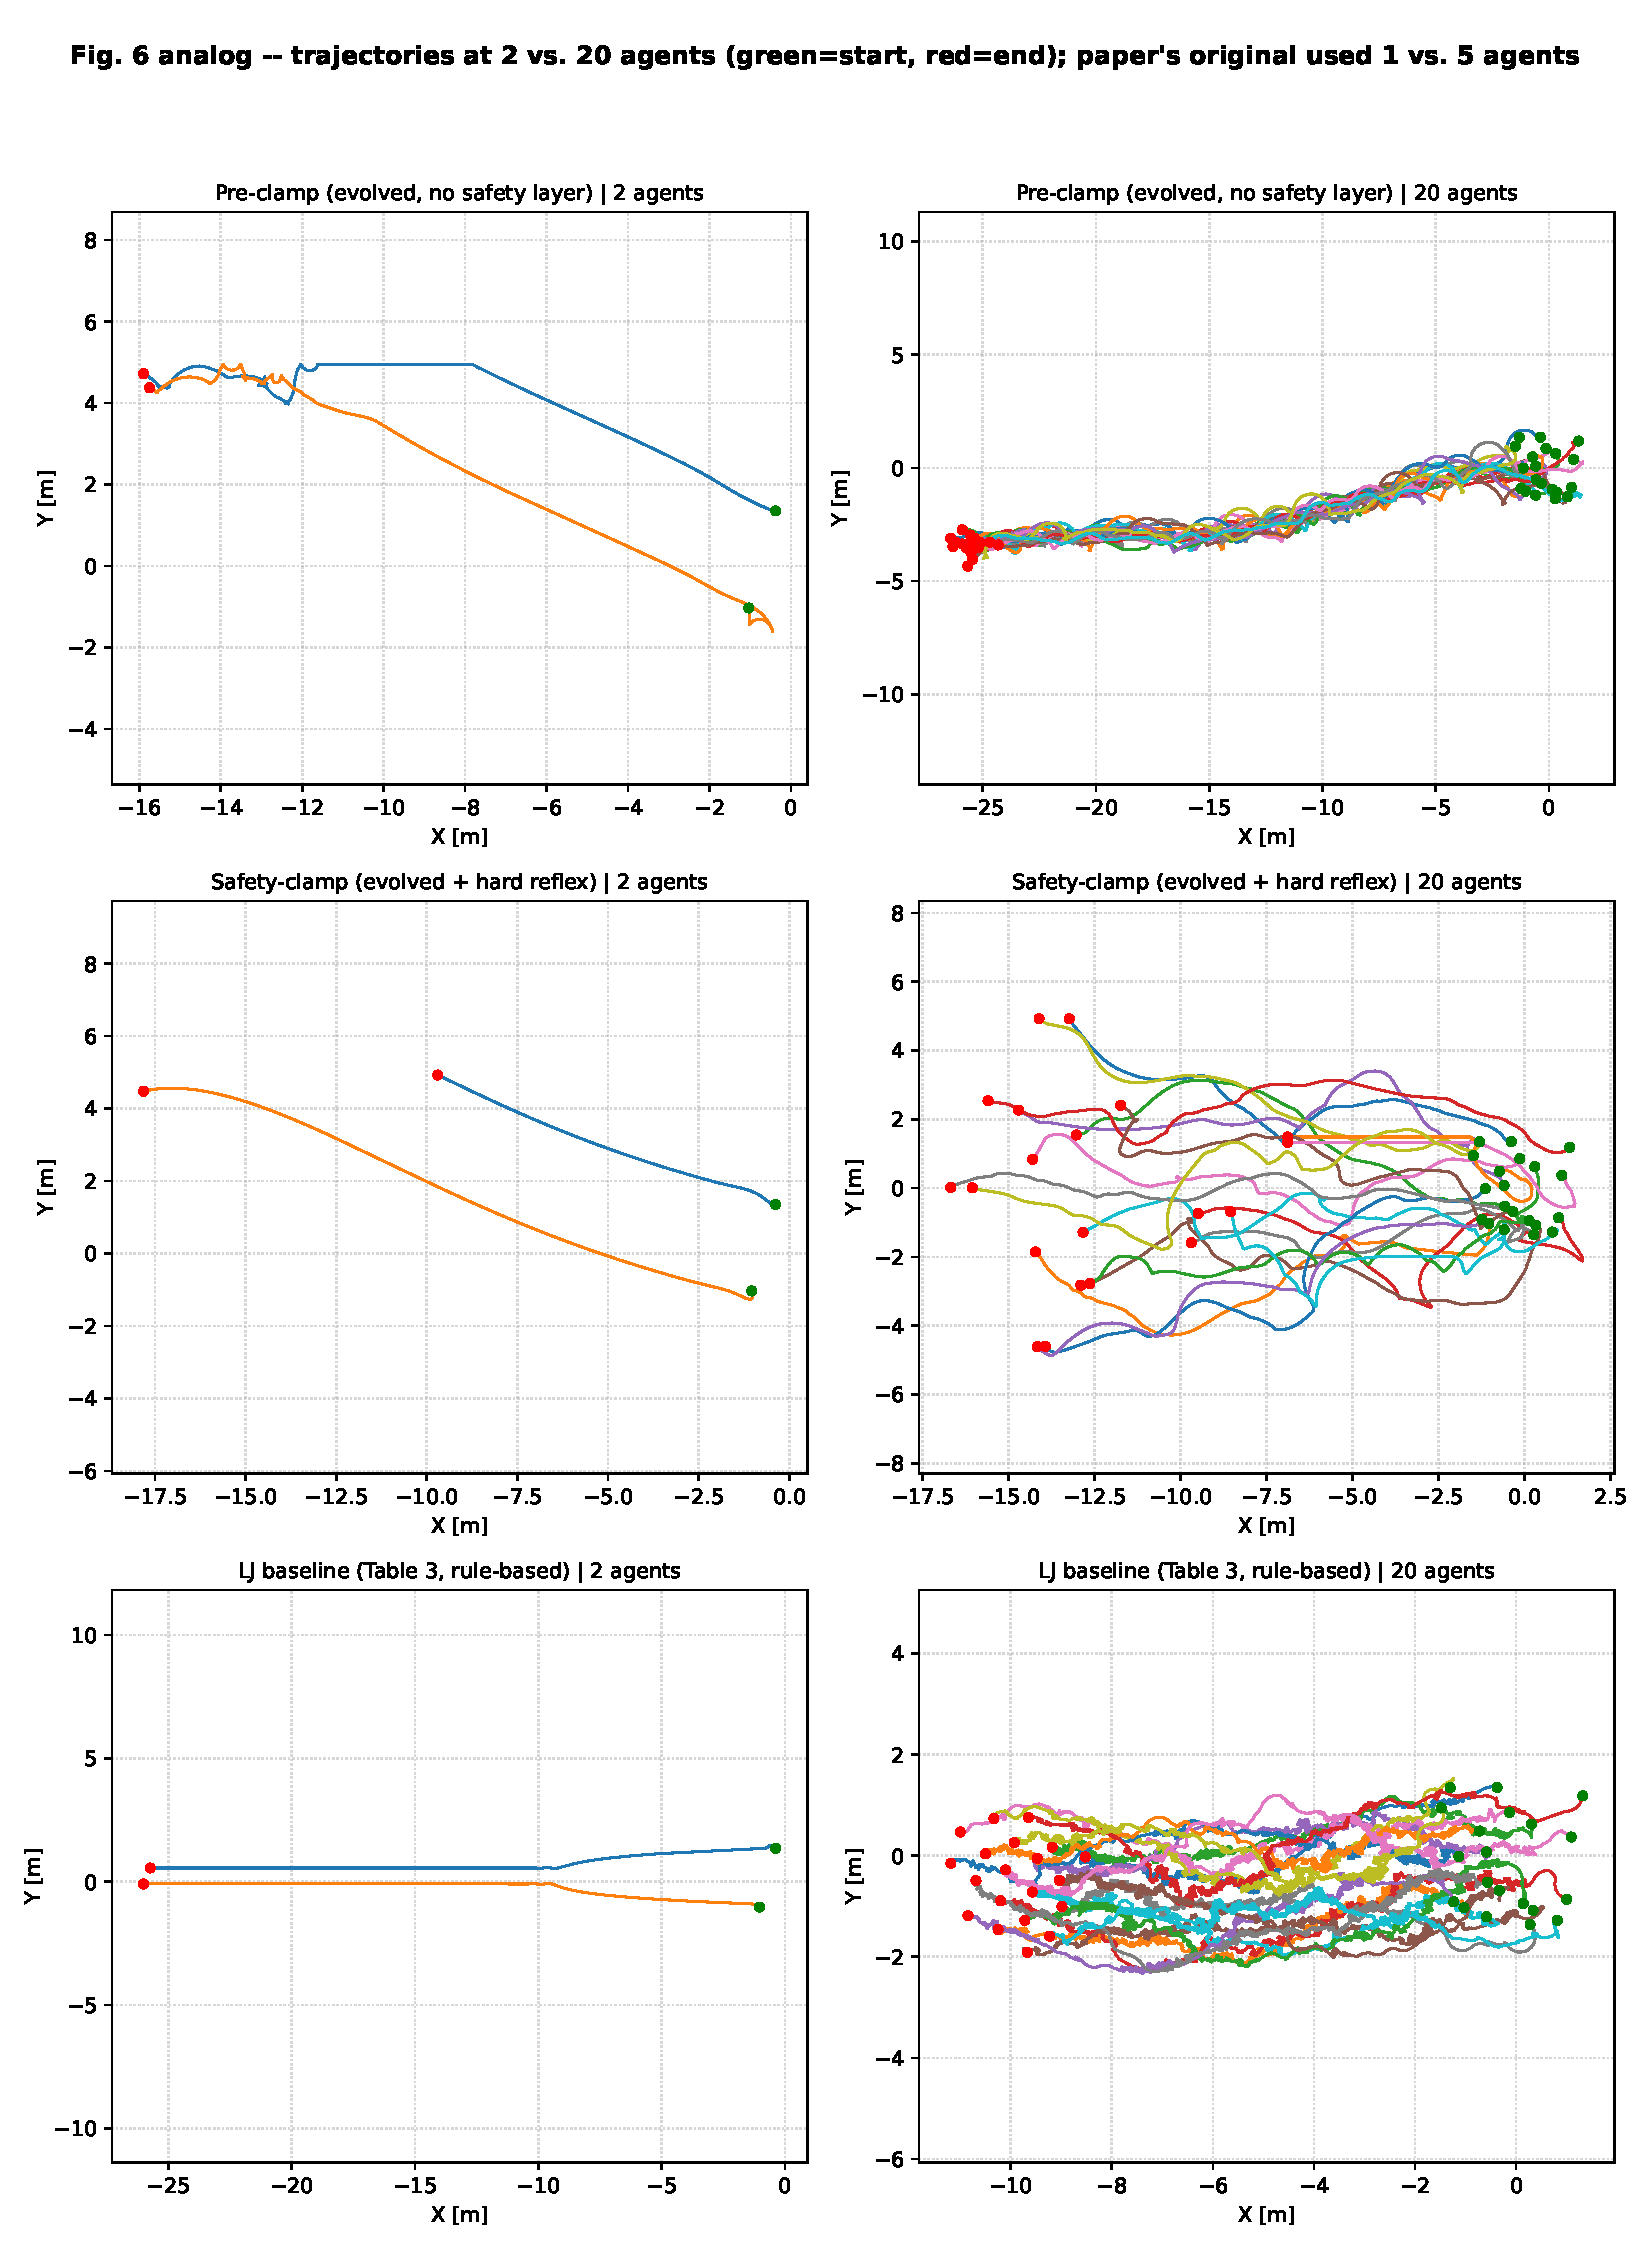
\includegraphics[width=\textwidth]{figures/paper_fig6_trajectory_comparison}
\caption{\textbf{Fig.~6 analog.} Trajectories at a small and a large swarm size (green = start,
red = end), seed 42. The paper's original figure compared 1 vs.\ 5 agents to argue that
formation reconfiguration is a collective, not individual, behavior;
\texttt{hardware\_transfer\_test} has no $n=1$ condition, so this uses $n=2$ vs.\ $n=20$
instead.}
\label{fig:fig6}
\end{figure}

\clearpage
\subsection{Metric 3 -- front-rank occupancy \& exchange rate}
\label{sec:metric3}

\begin{figure}[h]
\centering
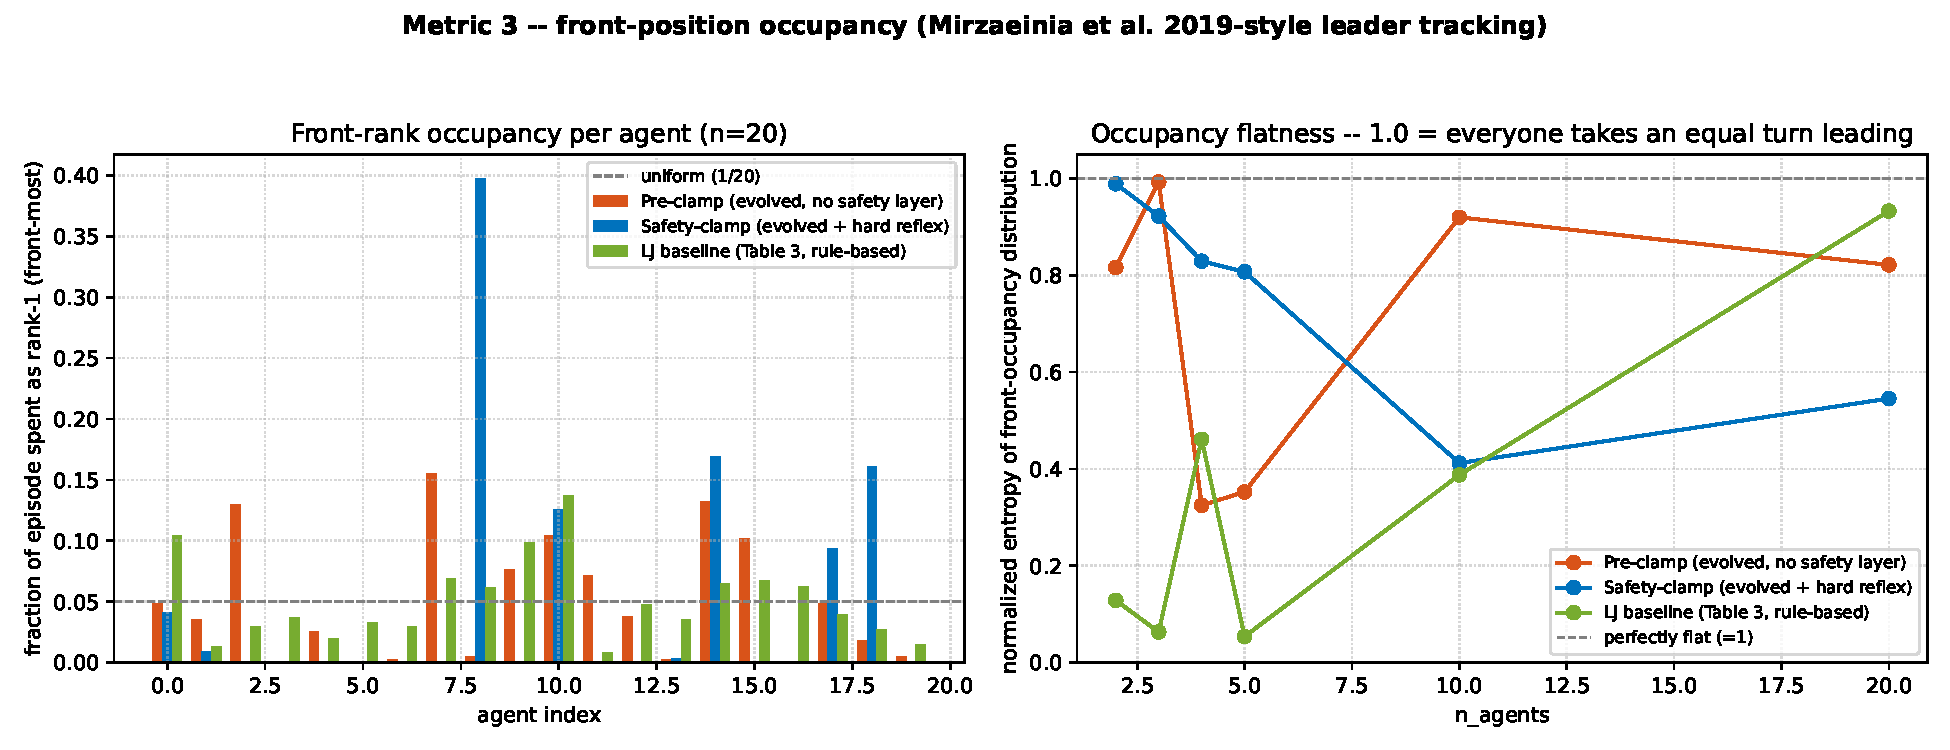
\includegraphics[width=\textwidth]{figures/metric3_front_occupancy}
\caption{Left: front-rank occupancy fraction per agent at $n=20$ (seed 42). Right: normalized
occupancy entropy vs.\ swarm size, per condition (1.0 = perfectly flat, i.e.\ every agent leads
an equal share of the episode).}
\end{figure}

\begin{figure}[h]
\centering
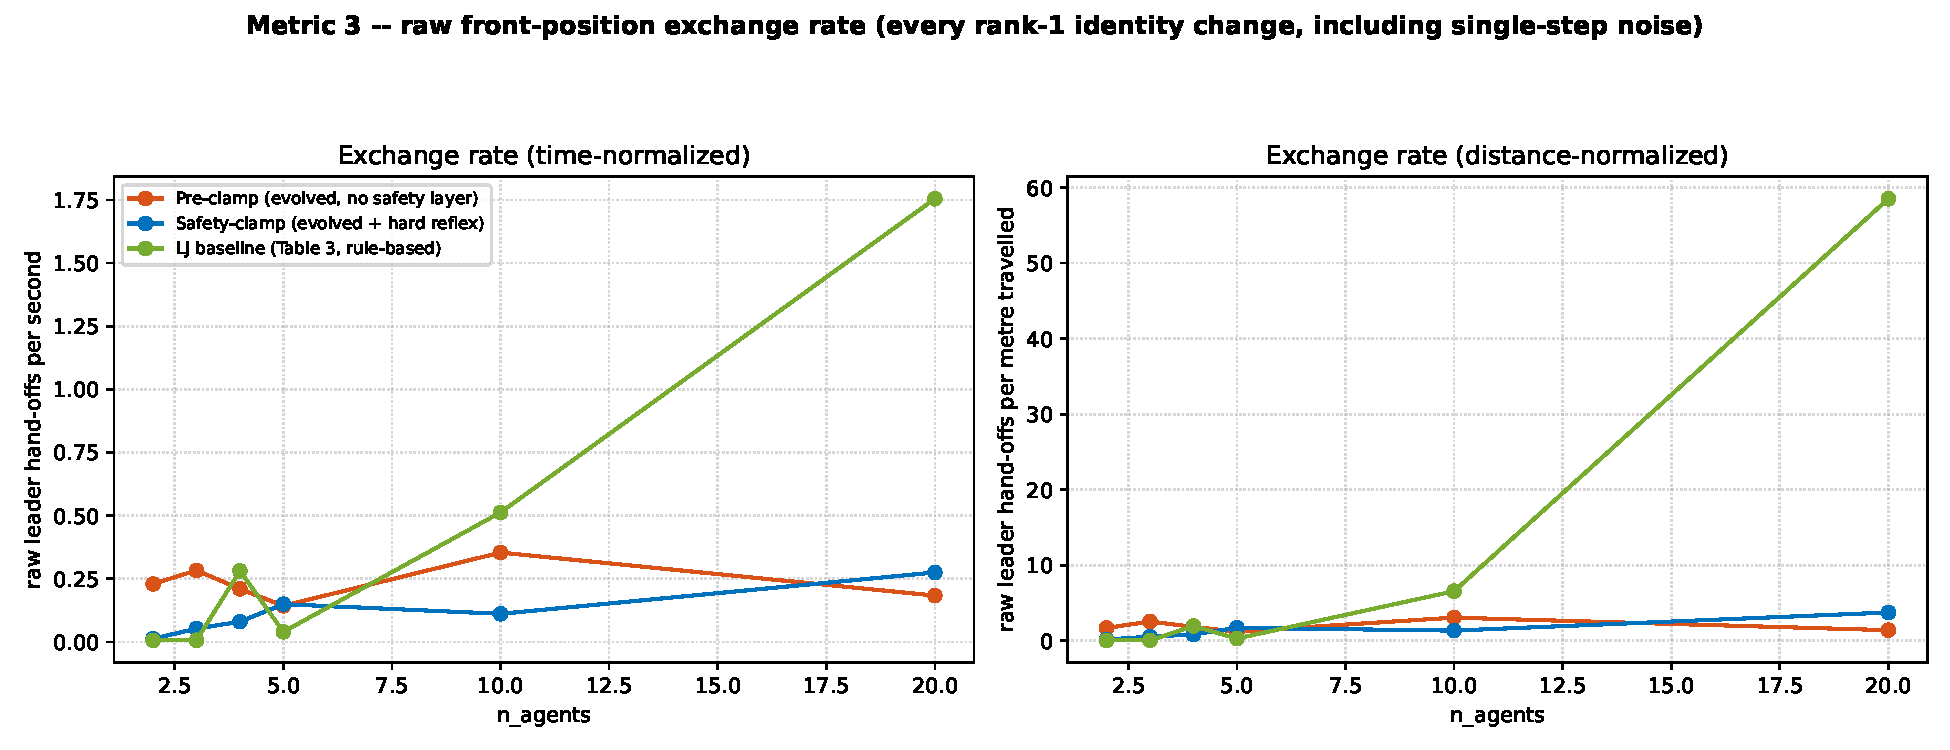
\includegraphics[width=\textwidth]{figures/metric3_exchange_rate}
\caption{Raw front-position exchange rate (every rank-0 identity change, including
single-step noise) vs.\ swarm size, time- and distance-normalized.}
\end{figure}

\begin{figure}[h]
\centering
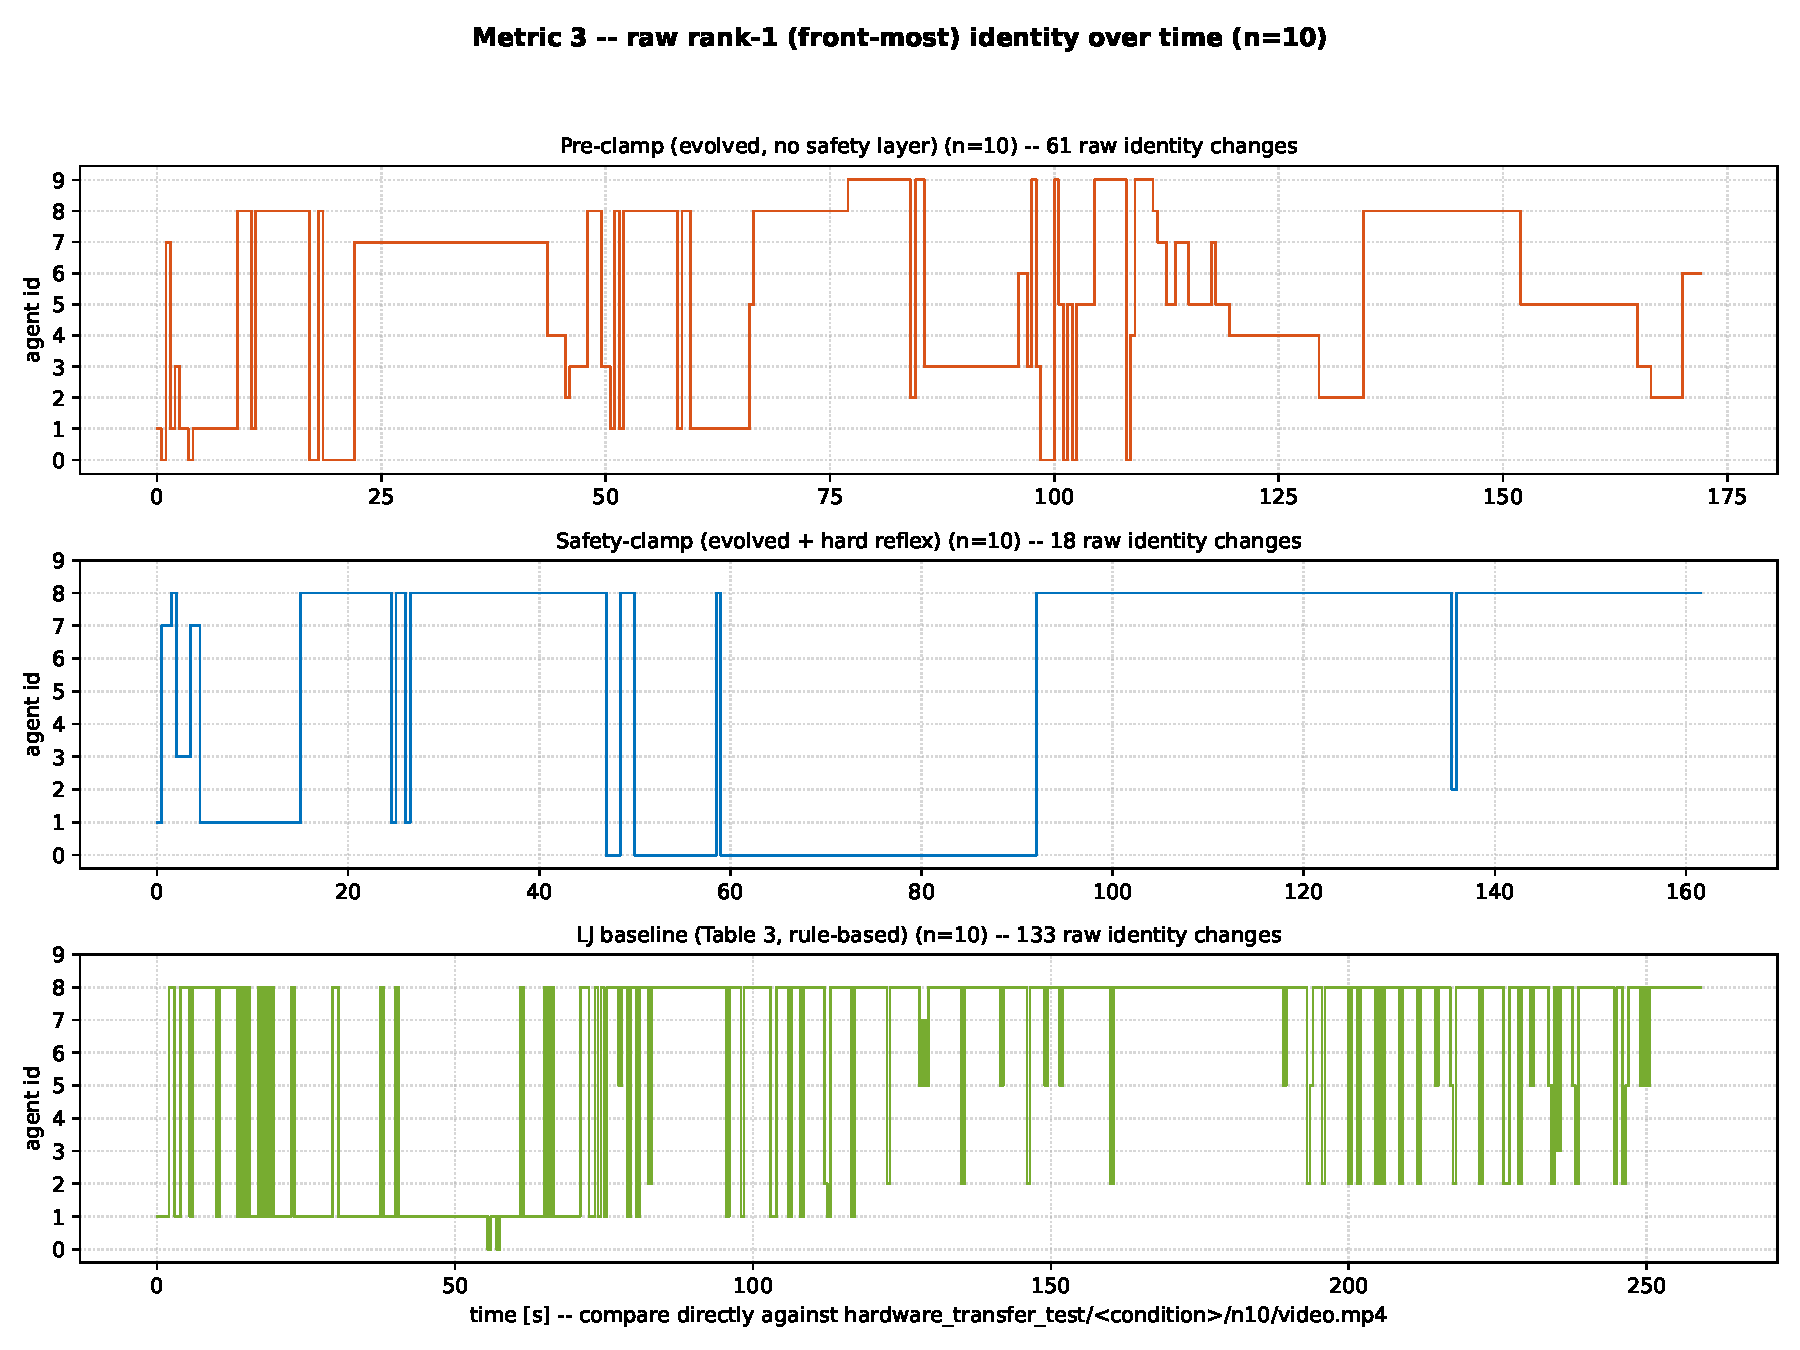
\includegraphics[width=0.9\textwidth]{figures/metric3_front_id_timeline_n10}
\caption{Raw rank-0 (front-most) agent identity over time, $n=10$, seed 42, one panel per
condition. Directly comparable against
\texttt{hardware\_transfer\_test/<condition>/n10/video.mp4}.}
\end{figure}

\begin{figure}[h]
\centering
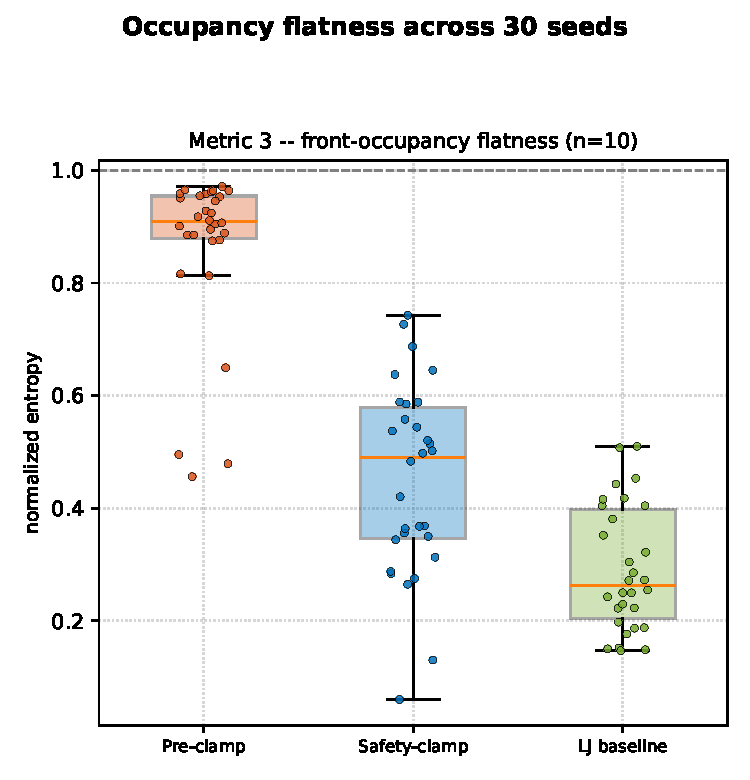
\includegraphics[width=0.7\textwidth]{figures/metric3_seed_sweep_n10}
\caption{Occupancy-flatness distribution across the 30-seed robustness sweep ($n=10$): box +
per-seed strip plot, one box per condition.}
\end{figure}

\clearpage
\subsection{Metric 4 -- persistence-filtered hand-off rate}
\label{sec:metric4}

\begin{figure}[h]
\centering
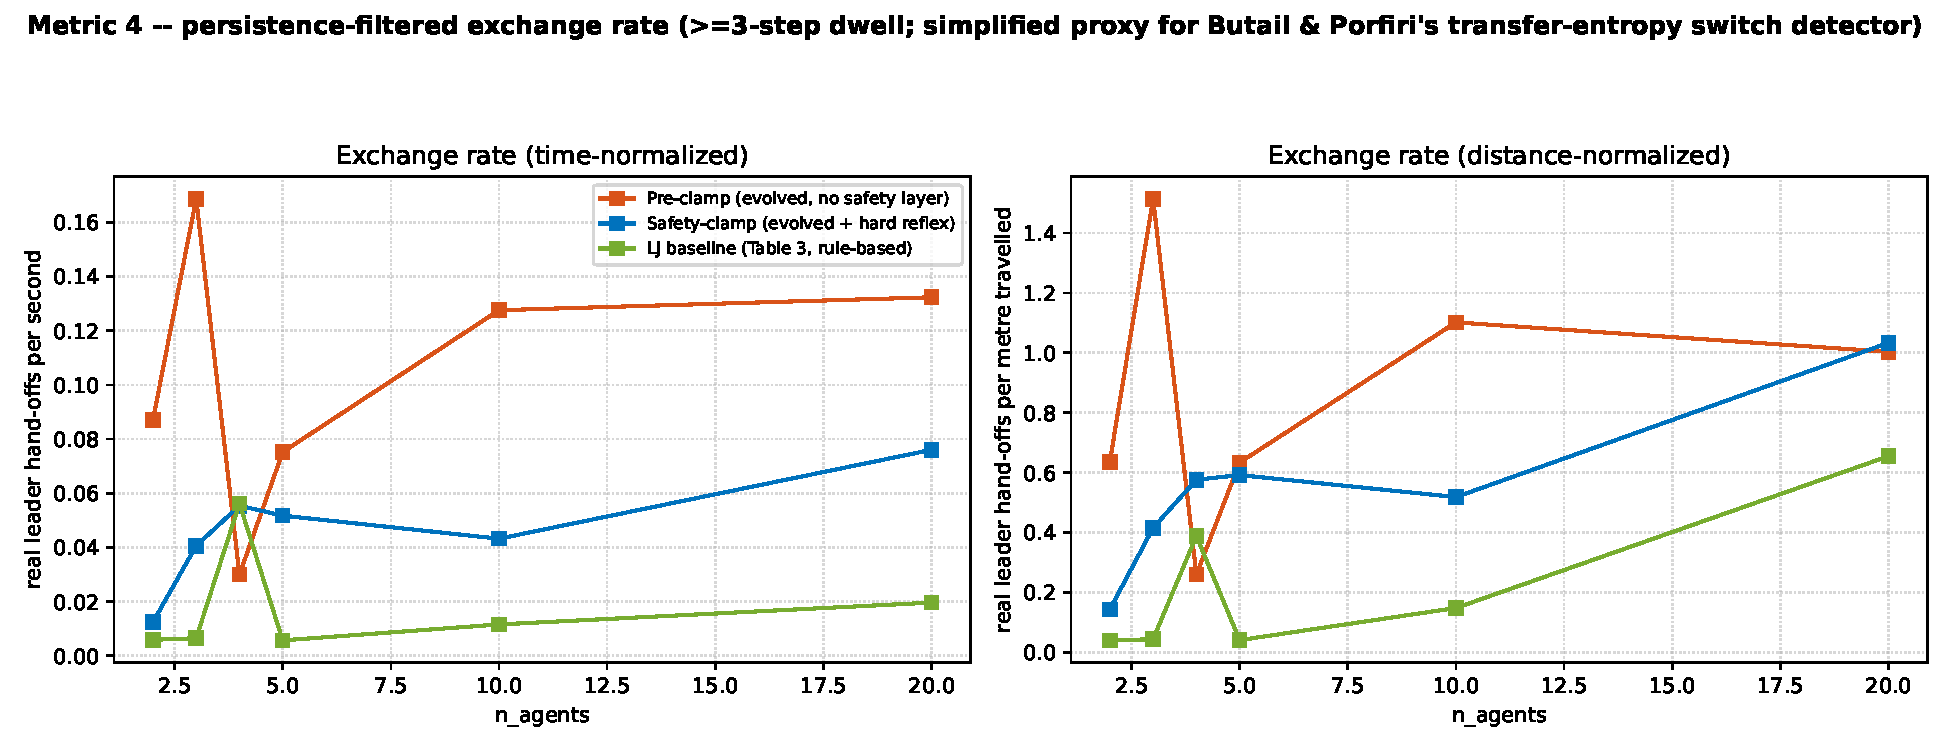
\includegraphics[width=\textwidth]{figures/metric4_exchange_rate_filtered}
\caption{Persistence-filtered ($\geq$3-step dwell) exchange rate vs.\ swarm size,
time- and distance-normalized. Compare directly against the raw exchange-rate plot in
Section~\ref{sec:metric3} -- the gap between the two is the fraction of raw switches that are
noise rather than genuine hand-offs.}
\end{figure}

\begin{figure}[h]
\centering
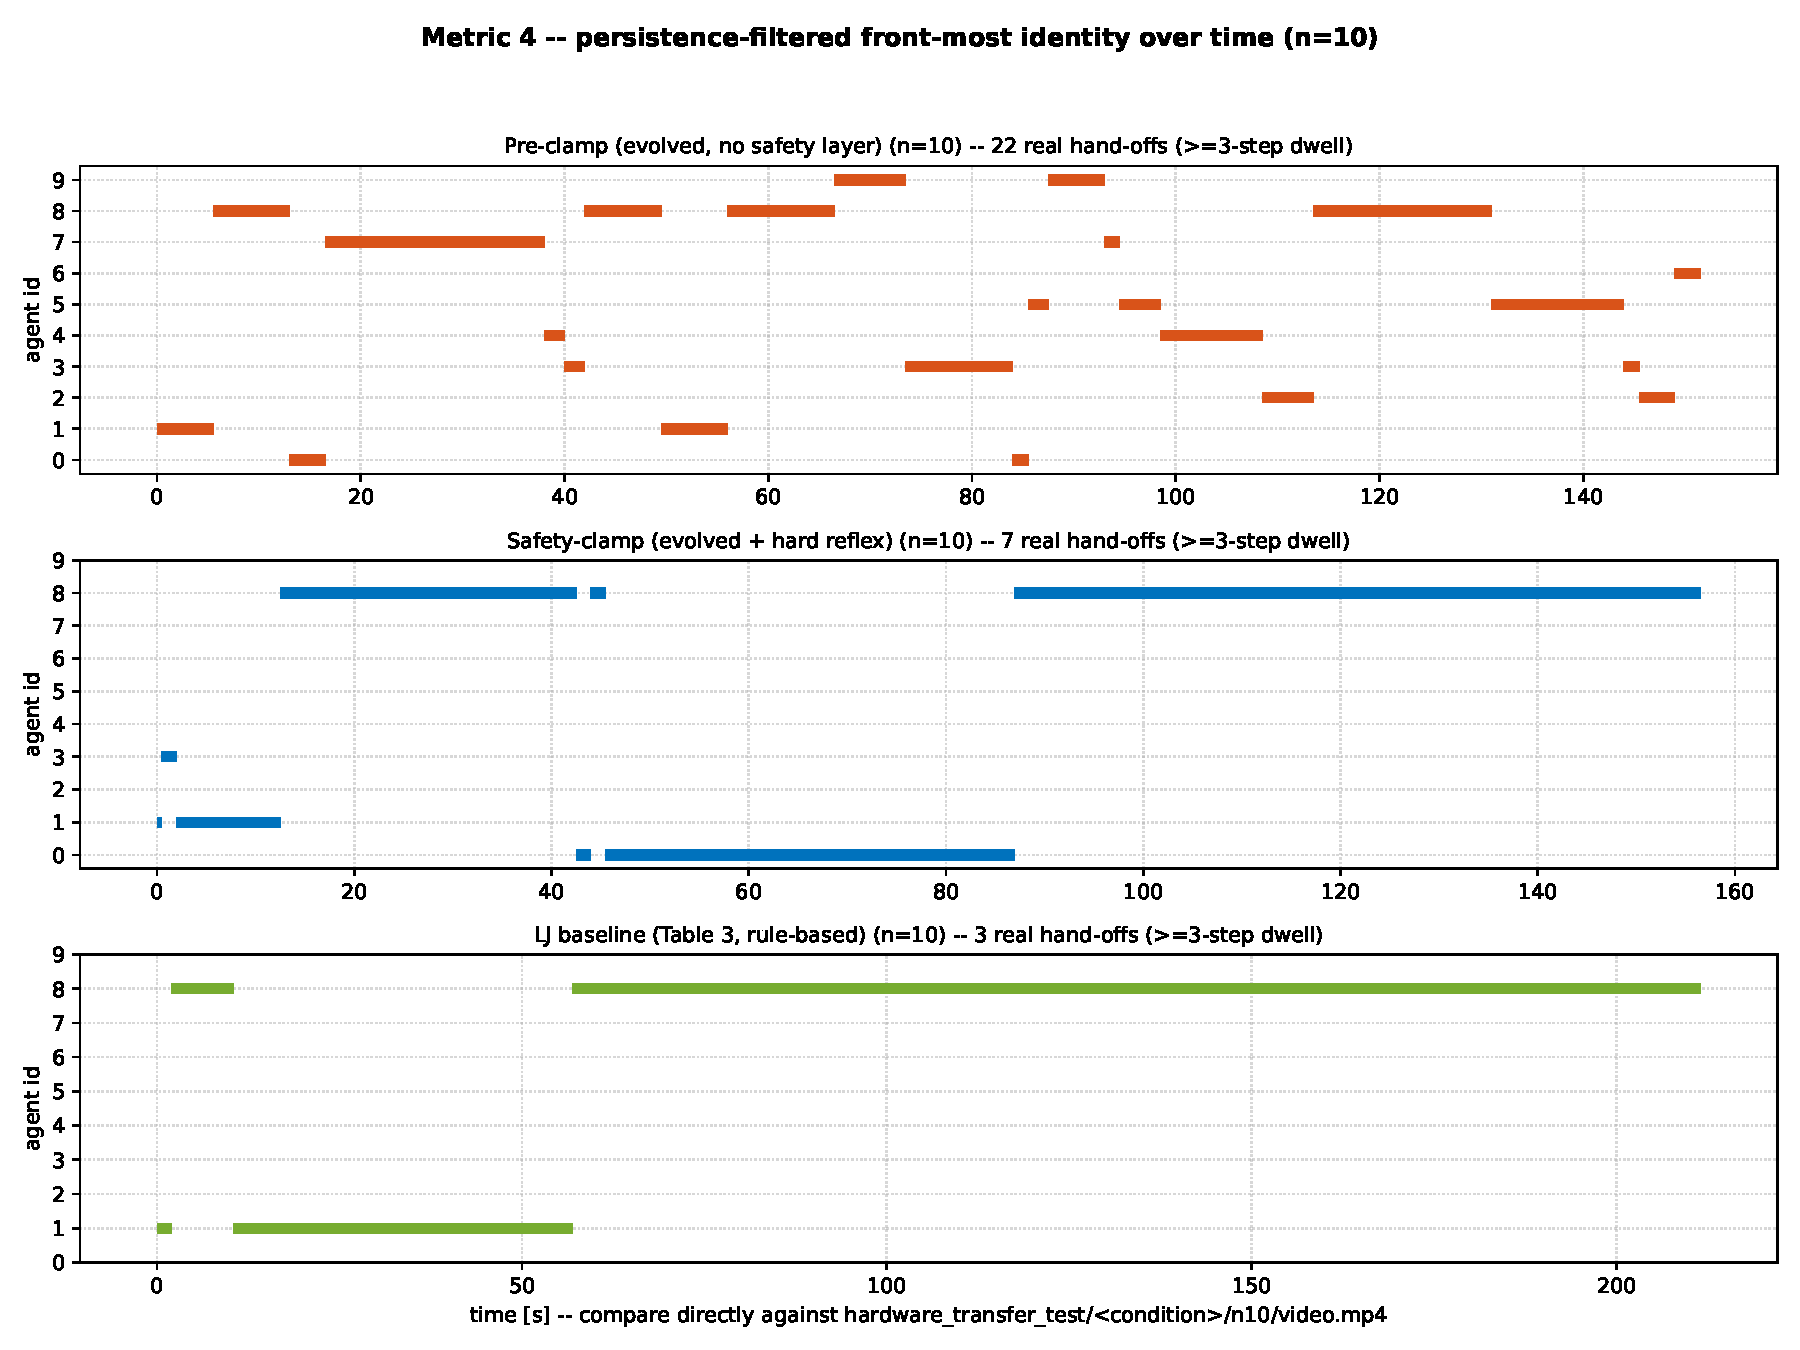
\includegraphics[width=0.9\textwidth]{figures/metric4_handoff_timeline_n10}
\caption{Persistence-filtered ``real'' leader segments over time, $n=10$, seed 42, same
episodes as the Metric~3 timeline above -- compare the two directly to see which raw switches
survive filtering.}
\end{figure}

\begin{figure}[h]
\centering
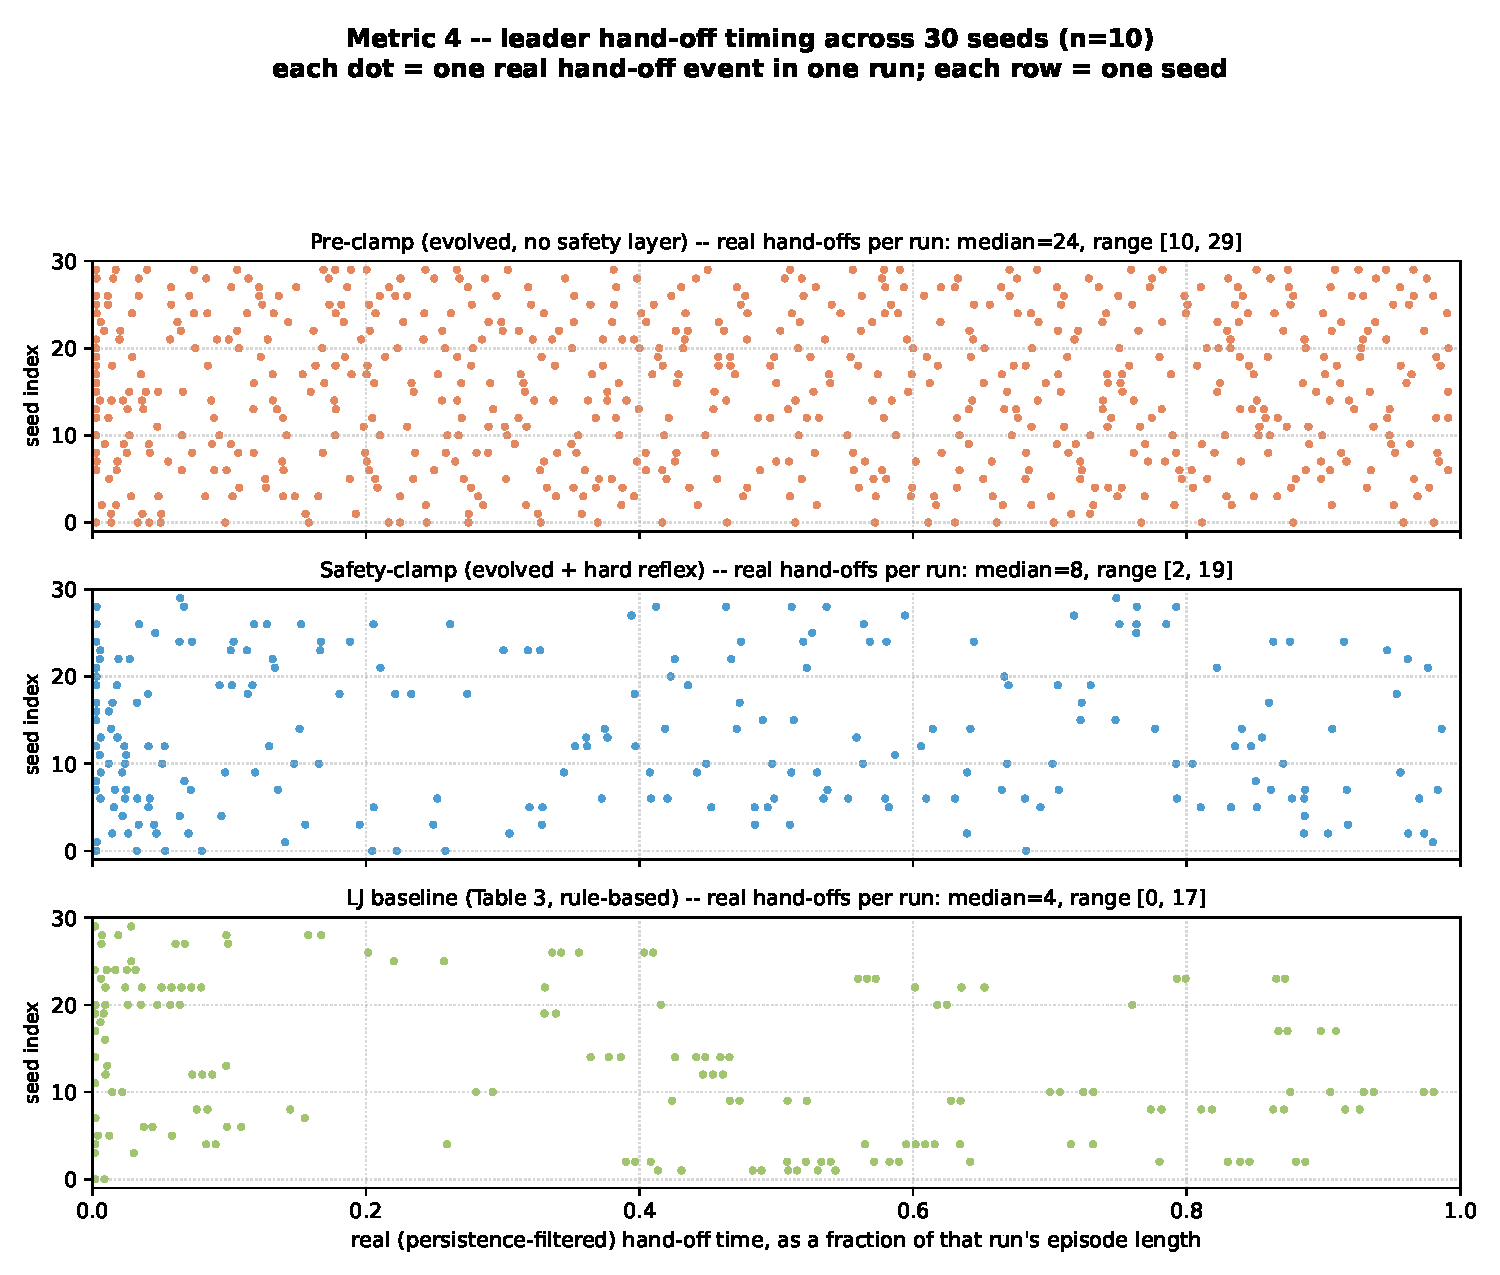
\includegraphics[width=0.85\textwidth]{figures/metric4_switch_event_raster_n10}
\caption{Real hand-off timing across the 30-seed robustness sweep ($n=10$): each dot is one
real hand-off event in one run, each row is one seed, x-axis is hand-off time as a fraction of
that run's episode length.}
\end{figure}

\begin{figure}[h]
\centering
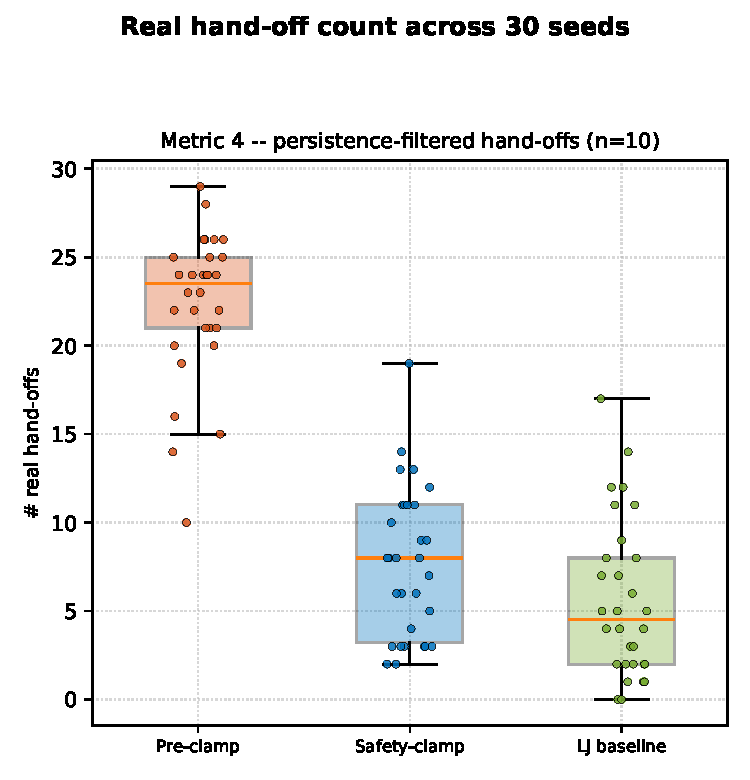
\includegraphics[width=0.7\textwidth]{figures/metric4_seed_sweep_n10}
\caption{Real hand-off count distribution across the 30-seed robustness sweep ($n=10$): box +
per-seed strip plot, one box per condition.}
\end{figure}

\clearpage
\begin{thebibliography}{9}

\bibitem{mahdavi2026}
Mahdavi et al.\ (2026). \emph{Energy-Efficient Flocking in Self-Organized Robot Swarms}. ANTS
2026 (PoliMi). \emph{[Complete with full author list / venue details / DOI once available; code
companion at \url{https://doi.org/10.5281/zenodo.18602800}.]}

\bibitem{mirzaeinia2019}
Mirzaeinia, A., et al.\ (2019). Greedy leading/trailing replacement heuristic for
energy-efficient UAV swarm flight.

\bibitem{butail2019}
Butail, S., Porfiri, M.\ (2019). Detecting switching leadership in collective motion.
\emph{Chaos}, 29(1), 011102.

\end{thebibliography}

\end{document}
